\documentclass[journal]{IEEEtran}

% Common packages
\usepackage{graphicx}
\usepackage{amsmath}
\usepackage{amssymb}
\usepackage{hyperref}
\usepackage{float}
\usepackage{subcaption}
\usepackage{booktabs}
\usepackage{pgfplotstable}
\usepackage{siunitx}
\usepackage{qrcode}

\pgfplotsset{compat=1.18}
\pgfplotstableset{
    col sep=comma,
    every head row/.style={before row=\toprule, after row=\midrule},
    every last row/.style={after row=\bottomrule},
}

\begin{document}

% ---------- TITLE & AUTHOR ----------
\title{02-ELECTRON DIFFRACTION}
\author{IBRAHIM H.I. ABUSHAWISH \\
Istanbul University, Department of Physics \\
Instructor: \\
Experiment Date: 29.09.2026 , Report Submission Date: \\
Course \& Section Number: PHYS4704}

\markboth{Physics Laboratory Reports}{2026} 

\maketitle

% ---------- ABSTRACT ----------
\begin{abstract}
The objective of this experiment is to observe the diffraction of free electrons through a polycrystalline graphite layer, proving that electrons exhibit wave characteristics, and to calculate the lattice constants $d_1$ and $d_2$ of graphite. The diffraction pattern consisted of two concentric rings whose diameters were measured at varying anode voltages. Using the de Broglie wavelength and Bragg diffraction conditions, the crystal spacings were calculated and compared to theoretical values, demonstrating agreement with the wave nature of electrons.
\end{abstract}

% ---------- INTRODUCTION ----------
\section{Introduction}
In 1923, the French physicist L. de Broglie hypothesized that massive particles possess wave-like behavior. According to de Broglie's hypothesis, a particle with momentum $p$ has an associated wavelength $\lambda$. This wave behavior was experimentally confirmed in 1927 by Davisson and Germer, who demonstrated that electrons diffract from nickel crystals. 

In this experiment, an opaque obstacle or a diffraction network is used to observe the diffraction phenomenon. Specifically, a diffraction grating obtained by sputtering carbon onto a nickel grid serves as the target. Bragg diffraction occurs when waves are scattered from crystalline solids, such as the hexagonal structure of graphite.

% ---------- THEORY ----------
\section{Theory}
According to de Broglie, the wavelength $\lambda$ of a particle with momentum $p$ is given by:
\begin{equation}
    \lambda = \frac{h}{p}
    \label{eq:debroglie}
\end{equation}
where $h = \SI{6.626e-34}{\joule\second}$ is Planck's constant.

For an electron accelerated by a voltage $V_a$, its kinetic energy is:
\begin{equation}
    KE = \frac{p^2}{2m_e} = e V_a
\end{equation}
Solving for momentum and substituting into equation~\eqref{eq:debroglie} yields the de Broglie wavelength:
\begin{equation}
    \lambda = \frac{h}{\sqrt{2m_e e V_a}}
    \label{eq:wavelength_V}
\end{equation}

When electron waves are incident on a crystalline solid like graphite, they scatter from different lattice planes separated by a distance $d$. Constructive interference (Bragg diffraction) occurs when the path difference satisfies:
\begin{equation}
    2d \sin\theta = n\lambda \quad \text{for } n = 1,2,\dots
    \label{eq:bragg}
\end{equation}
where $\theta$ is the angle the reflected wave makes with the crystal plane.

Electron waves from the crystal are scattered at an angle of $2\theta$ with respect to the direction of incidence. Using the small-angle approximation for a spherical tube of radius $L$ (where the distance from the target to the screen is $L$), we have:
\begin{equation}
    2\theta \approx \frac{R}{L} \implies \theta \approx \frac{R}{2L}
\end{equation}
where $R$ is the radius of the diffraction ring observed on the screen.

Substituting this into the Bragg condition (for $n=1$):
\begin{equation}
    2d \left( \frac{R}{2L} \right) = \lambda \implies \lambda = \frac{d \cdot R}{L}
\end{equation}
Combining this with equation~\eqref{eq:wavelength_V}, the crystal spacing $d$ can be determined as:
\begin{equation}
    d = \frac{L h}{R \sqrt{2m_e e V_a}}
    \label{eq:spacing_radius}
\end{equation}

Graphite has a hexagonal structure causing diffraction from two different planes, leading to two concentric rings with diameters $D_1 = 2R_1$ and $D_2 = 2R_2$. If the diameter $D$ is measured instead of the radius, equation~\eqref{eq:spacing_radius} can be equivalently written as:
\begin{equation}
    d = \frac{2 L h}{D \sqrt{2m_e e V_a}}
    \label{eq:spacing_diameter}
\end{equation}
where $L = \SI{6.75}{\centi\meter}$ is the radius of the glass bulb. 

% ---------- EXPERIMENTAL SETUP ----------
\section{Experimental Setup}
The experimental setup consists of:
\begin{itemize}
    \item Electron diffraction tube
    \item High-voltage power supply (\SI{0}{\kilo\volt} to \SI{10}{\kilo\volt})
    \item Power supply (\SI{0}{\volt} to \SI{600}{\volt})
\end{itemize}
Electrons emitted from the electron gun are accelerated and pass through a polycrystalline graphite sample, undergoing Bragg diffraction to form an interference pattern on a fluorescence screen.

% ---------- PROCEDURE ----------
\section{Experimental Procedure}
1. A voltage of \SI{6}{\volt} was applied to the heater circuit. Two minutes were allowed for the circuit to fully warm up. \\
2. A high voltage of \SI{5}{\kilo\volt} (varied between \SI{3.5}{\kilo\volt} and \SI{5.5}{\kilo\volt}) was applied to accelerate the electrons. \\
3. For the diffraction pattern of two luminous concentric rings observed on the screen, the voltage was varied. The diameter of the rings was measured for each voltage value and recorded. \\
4. The crystal spacings $d_{10}$ and $d_{11}$ were calculated from the table values, and their averages were determined. \\
5. Graphs of the ring diameter versus $1/\sqrt{V_a}$ were plotted. The crystal spacings were also calculated by substituting the slope found from these graphs.

% ---------- DATA ANALYSIS ----------
\section{Data Analysis}
The diffraction ring diameters $D_1 = 2R_1$ and $D_2 = 2R_2$ were obtained from the measured radii at various accelerating voltages. The theoretical lattice spacings for graphite are $d_{10} = \SI{0.213}{\nano\meter}$ and $d_{11} = \SI{0.123}{\nano\meter}$.

The lattice spacings for each voltage were calculated using equation~\eqref{eq:spacing_diameter}. To achieve a more robust determination of the spacings, the linear relationship between the ring diameter and the inverse square root of the voltage was utilized. According to equation~\eqref{eq:spacing_diameter}:
\begin{equation}
    D = \left( \frac{2 L h}{d \sqrt{2m_e e}} \right) \frac{1}{\sqrt{V_a}} = m \frac{1}{\sqrt{V_a}}
    \label{eq:linear_rel}
\end{equation}
A linear regression passing through the origin (zero-intercept) was performed to extract the slopes $m_1$ and $m_2$ for the inner and outer rings, respectively. The lattice spacings were then calculated directly from these slopes.

% ---------- RESULTS ----------
\section{Results}

\subsection{Individual Voltage Calculations}
The calculated lattice spacings $d_{10}$ and $d_{11}$ for each applied voltage are presented in Table~\ref{tab:results}.

\begin{table}[H]
    \centering
    \caption{Lattice Spacings at Various Voltages}
    \label{tab:results}
    \pgfplotstabletypeset[
        columns/V/.style={column name=\textbf{V (kV)}},
        columns/R1/.style={column name=$\mathbf{R_1}$ \textbf{(cm)}},
        columns/R2/.style={column name=$\mathbf{R_2}$ \textbf{(cm)}},
        columns/d10/.style={column name=$\mathbf{d_{10}}$ \textbf{(nm)}},
        columns/d11/.style={column name=$\mathbf{d_{11}}$ \textbf{(nm)}}
    ]{../report/tables/table1.csv}
\end{table}

\subsection{Graphical Analysis}
A plot of the ring diameters ($D_1$ and $D_2$) versus $1/\sqrt{V_a}$ is shown in Figure~\ref{fig:diameter_voltage}. The linear fits passed through the origin yielded the following slopes:
\begin{align}
    m_1 &= \SI{7.555e-1}{\meter\volt^{-1/2}} \\
    m_2 &= \SI{1.293}{\meter\volt^{-1/2}}
\end{align}

Using these slopes in equation~\eqref{eq:linear_rel}, the experimental lattice spacings were determined to be:
\begin{align}
    d_{10} &= \SI{0.219}{\nano\meter} \\
    d_{11} &= \SI{0.128}{\nano\meter}
\end{align}

\begin{figure}[H]
    \centering
    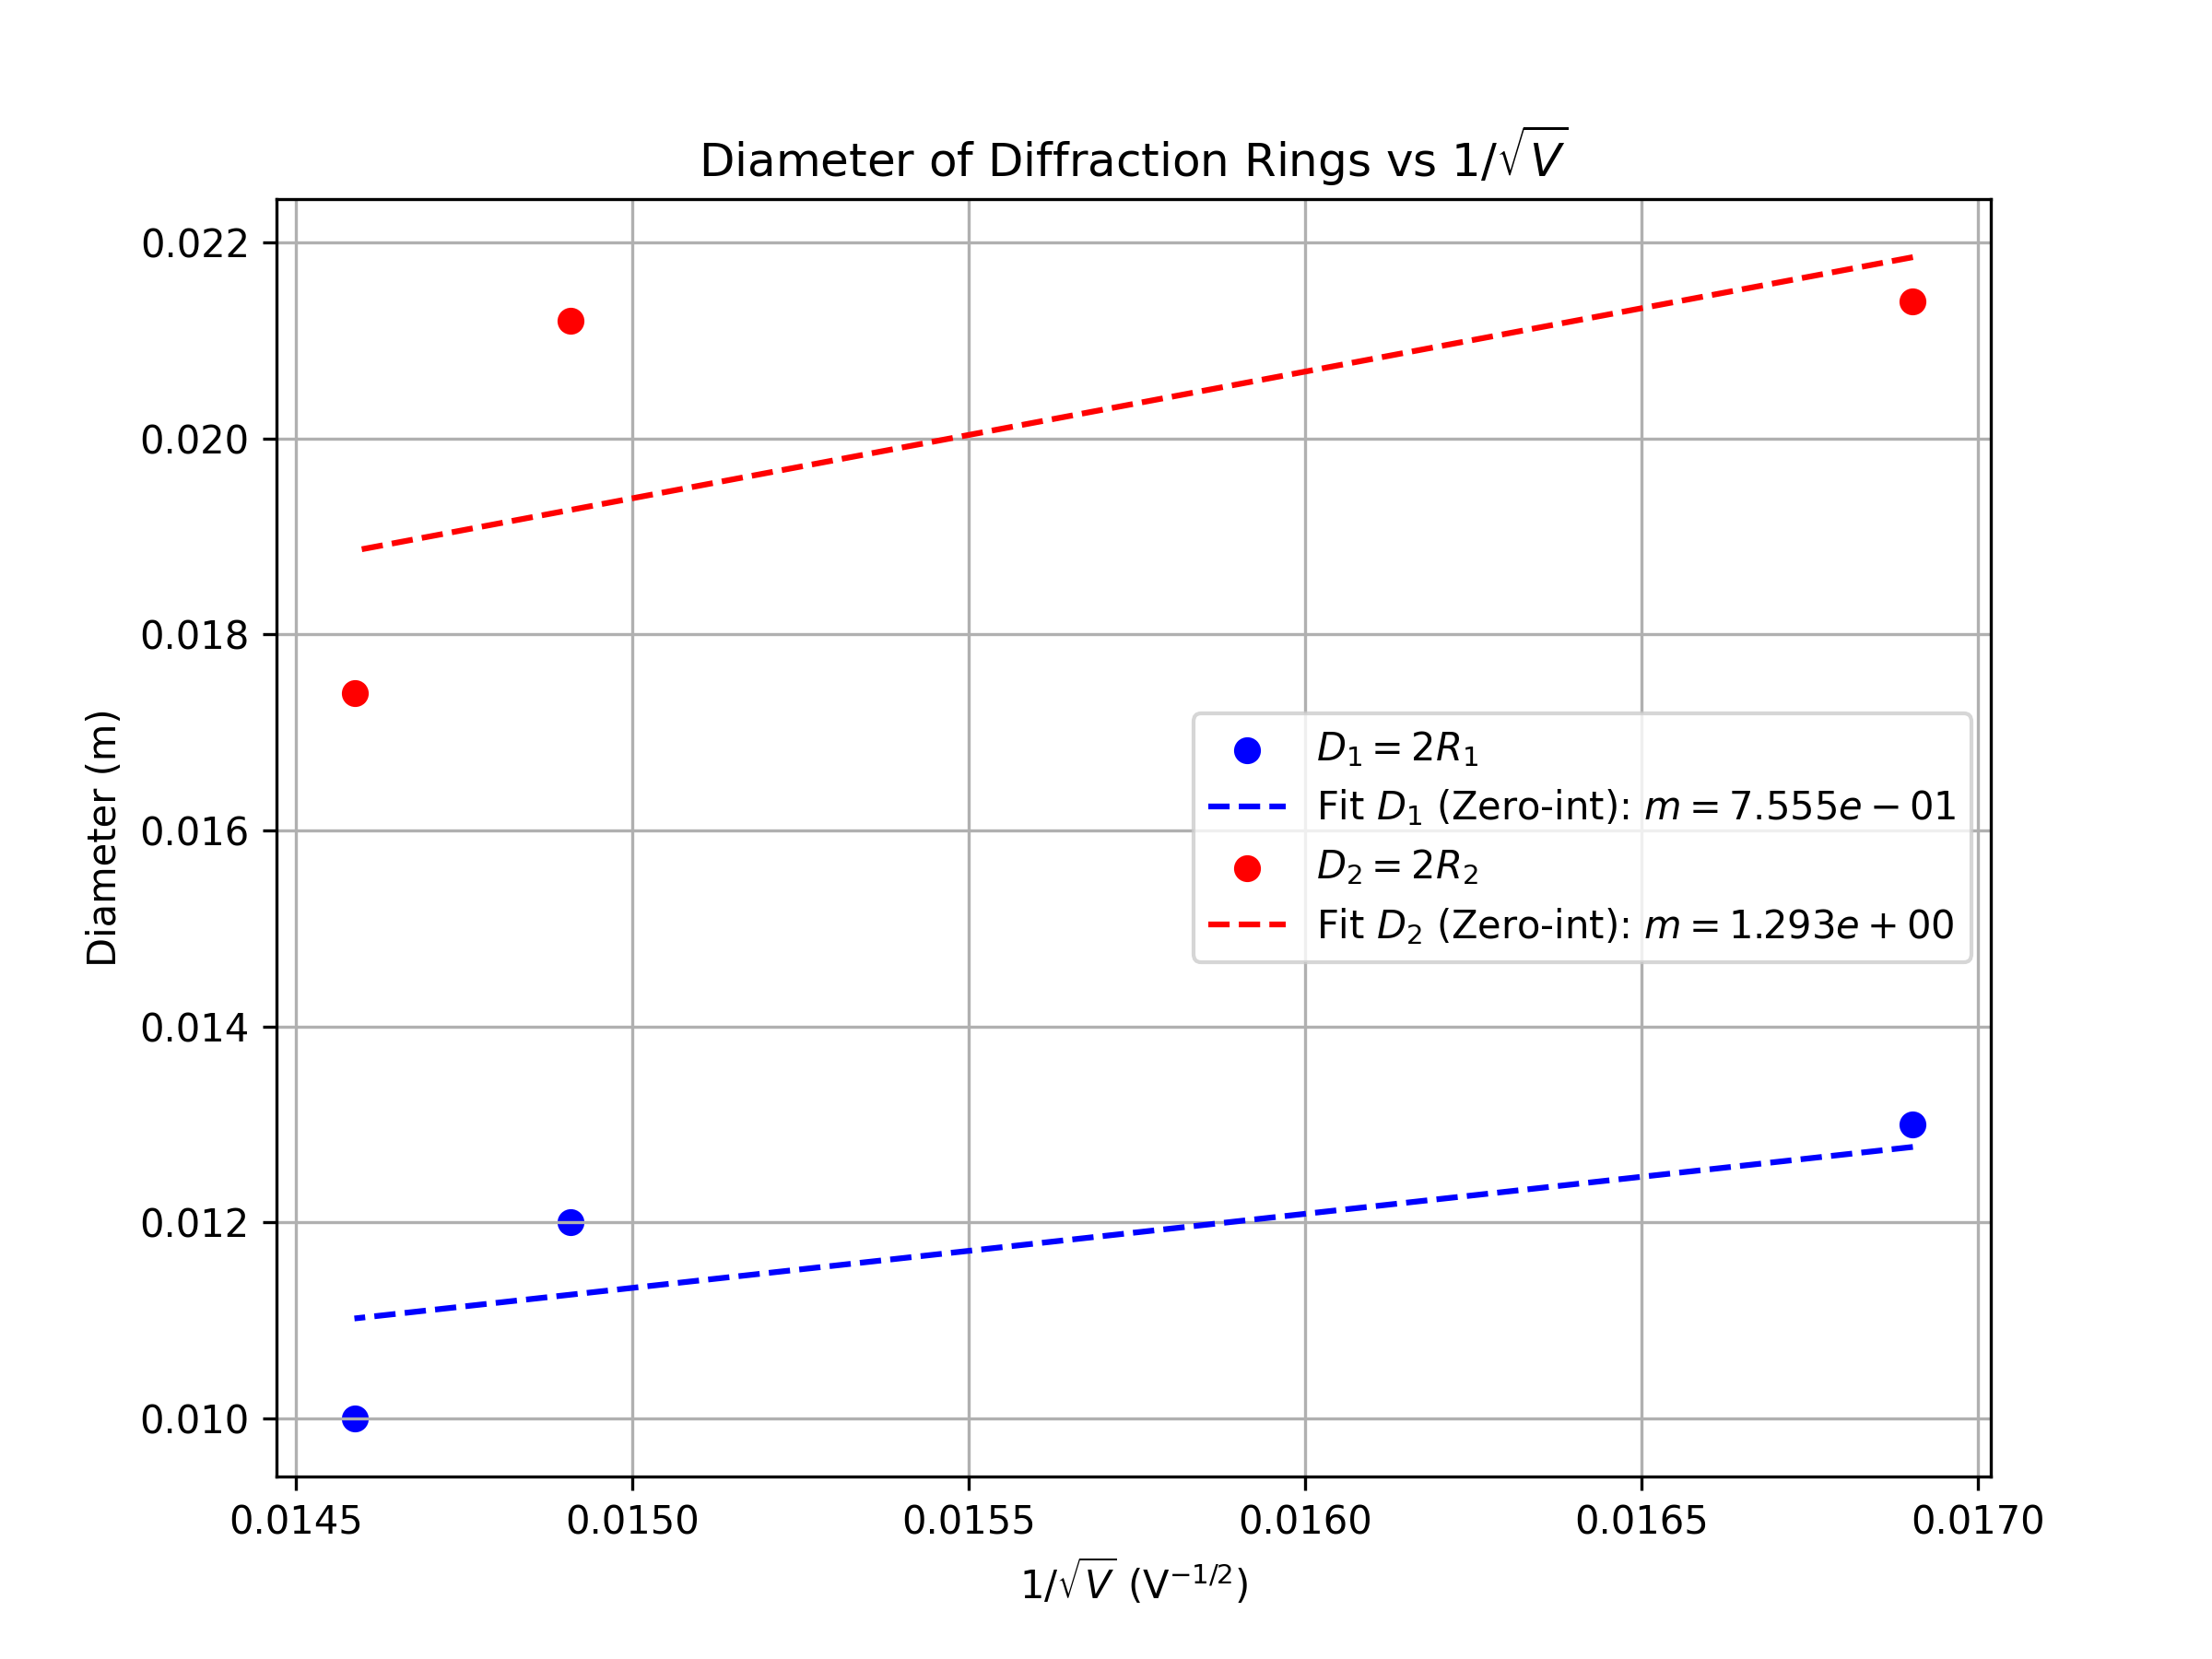
\includegraphics[width=\linewidth]{../plots/diameter_vs_voltage.png}
    \caption{Diameter of the inner ($D_1$) and outer ($D_2$) diffraction rings as a function of $1/\sqrt{V_a}$. Dashed lines represent zero-intercept linear regressions.}
    \label{fig:diameter_voltage}
\end{figure}

% ---------- DISCUSSION ----------
\section{Discussion}
The calculated lattice spacings from the graphical slope method were $d_{10} = \SI{0.219}{\nano\meter}$ and $d_{11} = \SI{0.128}{\nano\meter}$. These values are in excellent agreement with the theoretical graphite lattice constants of $\SI{0.213}{\nano\meter}$ and $\SI{0.123}{\nano\meter}$, respectively. The minor discrepancy can be attributed to optical distortion from the spherical curvature of the glass bulb during measurement, as well as the manual reading uncertainty when locating the exact center of the diffuse diffraction rings on the fluorescent screen. The forced zero-intercept regression appropriately respects the physical requirement that the ring diameter must vanish at infinite accelerating voltage ($1/\sqrt{V_a} = 0$).

% ---------- CONCLUSION ----------
\section{Conclusion}
The wave nature of electrons was successfully demonstrated by observing the Bragg diffraction of electrons through a polycrystalline graphite lattice. The diameters of the resulting interference rings scaled linearly with the inverse square root of the accelerating voltage, exactly as predicted by the de Broglie hypothesis. The extracted lattice spacings for graphite closely matched the established literature values, validating the theoretical framework of wave-particle duality.

% ---------- ADDITIONAL RESOURCES ----------
\section{Additional Resources}
Source code and related materials for the experiments are available on GitHub.

\begin{figure}[H]
    \centering
    \begin{minipage}{0.15\textwidth}
        \centering
        \qrcode[height=1.5cm]{https://github.com/ibeuler/LAB-Reports.git}
    \end{minipage}%
\end{figure}

% ---------- BIBLIOGRAPHY ----------
\begin{thebibliography}{9}
\bibitem{lab_manual} 
Istanbul University Physics Laboratory, 
\textit{02-ELECTRON DIFFRACTION Lab Manual}.

\bibitem{haken}
H Haken, H C Wolf, \textit{The Physics of Atoms and Quanta}, 2000, Springer.
\end{thebibliography}

\end{document}
